\documentclass[twocolumn]{article}

%Packages
\usepackage{amsmath}
\usepackage{amstext}
\usepackage{amssymb}
\usepackage{appendix}
\usepackage{coseoul}
\usepackage{enumerate}
\usepackage{graphicx}
\usepackage{import}
\usepackage{lscape}
\usepackage{modular}

\usepackage[pdfpagemode=UseNone,pdfstartview=FitH,colorlinks=true,linkcolor=blue,citecolor=blue,urlcolor=blue]{hyperref}
\usepackage[all]{hypcap}


% General physics constructs
\newcommand{\bra}[1]{\langle #1 |}
\newcommand{\ket}[1]{| #1 \rangle }
\newcommand{\braket}[2]{\langle #1|#2\rangle}
\newcommand{\bbraket}[3]{ \langle #1 | #2 | #3 \rangle }
\newcommand{\norm}[1]{\| #1\|}
\newcommand{\avg}[1]{\left \langle #1 \right \rangle}
\newcommand{\angavg}[1]{\left \langle #1 \right \rangle}
\newcommand{\abs}[1]{\left \lvert #1 \right \rvert}
\newcommand{\VS}{\textit{\textbf{V}}}
\newcommand{\Tr}{\textrm{Tr}}
\renewcommand{\Re}{\textrm{Re}}
\renewcommand{\Im}{\textrm{Im}}
\newcommand{\basis}[1]{\{\ket{#1}\}}

\newcommand{\omegaqubit}{\omega_{10}}

% Figures. Example usage:
% \quickfig{\columnwidth}{my_image}{This is the caption}{fig:my_fig}
\DeclareRobustCommand{\quickfig}[4]{
\begin{figure}
\begin{centering}
\includegraphics[width=#1]{#2}
\par\end{centering}
\caption{#3}
\label{#4}
\end{figure}
}

\DeclareRobustCommand{\quickwidefig}[4]{
\begin{figure*}[h]
\begin{centering}
\includegraphics[width=#1]{#2}
\par\end{centering}
\caption{#3}
\label{#4}
\end{figure*}
}


\title{Discrete Fourier Transform for Experimental Data}
\author{Daniel Sank\\\small{University of California, Santa Barbara}\\\small{Presently Google Quantum AI}}
\date{22 October, 2009}

\begin{document}

\maketitle

\begin{abstract}
Spectral analysis of data requires the use of the discrete Fourier
transform (DFT). In this note I will discuss the most basic and important
formulas needed to go from a time series of measured data values to
power spectrum with correct physical units. 
\end{abstract}


\section{The Four Fourier Transforms}

There are four different types of Fourier transform, corresponding
to the four different ways in which data may be sampled in time: data
may be known at discrete or continuous times, and over a finite or
infinite extent of time. The four transforms are 
\begin{itemize}
\item Fourier transform (FT) - continuous time, infinite extent 
\item Fourier series (FS) - continuous time, finite extent 
\item Discrete time Fourier transform (DTFT) - discrete time, infinite extent 
\item Discrete Fourier transform (DFT) - discrete time, finite extent 
\end{itemize}
Each of these transforms is useful in making calculations and in developing theoretical understanding, but in the lab where we have discretely sampled or generated data over finite durations of time, only the DFT really applies.


\section{DFT basics}

From the strictly mathematical point of view a series of experimental data is characterized by only one parameter, the number of points in the time series, which we denote by $N$.
Any mathematical formulae we develop should involve only this one parameter.

\subsection{Definition}

Consider a time series of data written as $x(n)$ where $n \in [0,\dots,N-1]$ labels the discrete time axis.
The DFT, like all Fourier transforms, is based on the fact that $x(n)$ can be written as a sum of exponentials,
\begin{equation}
x(n)=\frac{1}{N}\sum_{k=0}^{N-1}X(k)\, e^{i2\pi nk/N} \label{eq:iDFT_def}
\end{equation}
where the complex weights $X(k)$ are given by
\begin{equation}
X(k)=\sum_{n=0}^{N-1}x(n)\, e^{-i2\pi nk/N} \label{eq:DFT_def}
\end{equation}
These formulae can be shown to be consistent by substituting (\ref{eq:DFT_def}) into  into (\ref{eq:iDFT_def}).
The indices $n$ and $k$ run from $0$ to $N-1$ which we call the \textbf{baseband}.
The pair of equations (\ref{eq:iDFT_def}) and (\ref{eq:DFT_def}) are not the only way to define the DFT.
The only requirements are that the product of the prefactors of the two sums is $1/N$ and the signs of the exponentials are opposite.
Our choice to to put the factor of $1/N$ in the first equation matches the choice made in numpy and Matlab.
The various numerical packages in various programming languages use different conventions, so make sure to always check this before writing a program using any particular DFT.
Formulas given below assume the DFT specified by equations (\ref{eq:iDFT_def}) and (\ref{eq:DFT_def}), but the appropriate modifications of these for various DFT conventions should be clear once you understand the present case.


\subsection{General Properties}

Here we list the most important properties of the DFT. 

\subsubsection{Fourier frequencies}

From equation (\ref{eq:iDFT_def}) we see that our signal $x(n)$ is built up of exponentials $\exp(i2\pi nk/N)$.
We call the frequency $k/N$ the $k^{th}\textbf{ Fourier frequency}$.
The minimum Fourier frequency is 0 and the greatest is $(N-1)/N\approx1$.
These frequencies are in ``index units,'' meaning that the exponential $\exp(i 2 \pi n k / N)$ goes through $k/N$ oscillations per step of the index $n$.
Note that a Fourier frequency of 1 (which is \emph{not} in the baseband) is actually just a constant function; if the signal goes through exactly one cycle per index, it attains the same value at each index.


\subsubsection{All information in baseband}

A signal $x(n)$ is completely determined by knowledge of $X(k)$ for $k$ in the baseband $[0,\ldots,N-1]$.
Still, if we have a series $x(n)$ in hand and we regard equation (\ref{eq:DFT_def}) as a formula that spits out $X(k)$ for $\emph{any}$ integer $k$, we can compute $X(k)$ for $k$ outside the baseband.
However, these new $X(k)$'s are not independent of the ones in the baseband.
To see this, first note that any integer $k$ can be written as $k=p+mN$ where $p \in [0..N-1]$ and $m$ is an integer, as shown in Figure \ref{fig:baseband}.
Note that if $m=0$ then $k=p$ and $k$ is in the baseband, and if $m \neq 0$ then $k$ is not in the baseband.
Computing the DFT we find
\begin{align}
X(k) &= \sum_{n=0}^{N-1} x(n) e^{-i2\pi nk/N}\\
&= \sum_{n=0}^{N-1} x(n) e^{-i2\pi np/N} e^{-i2\pi nm} \\
&= \sum_{n=0}^{N-1} x(n)e^{-i2\pi np/N} \\
&= X(p) \, .
\end{align}
The DFT computed for $k$ is exactly equal to the DFT computed for $p$.
This means that, given a series $x(n)$, only the weights $X(k)$ are uniquely determined only for $k \in [0, \ldots , N-1]$.
In other words, all of the information about the original series $x(n)$ is contained in the set $X(k)$ for $k$ in the baseband.
Fourier coefficients can be computed for $k$ outside this range, but they are all related to the ones in the baseband by translation in $k$ space:
\begin{equation}
X(k) = X(k+mN) \quad \textrm{for all integers }m \, . \label{eq:translational_symmetry}
\end{equation}

\begin{figure*}[t]
\begin{centering}
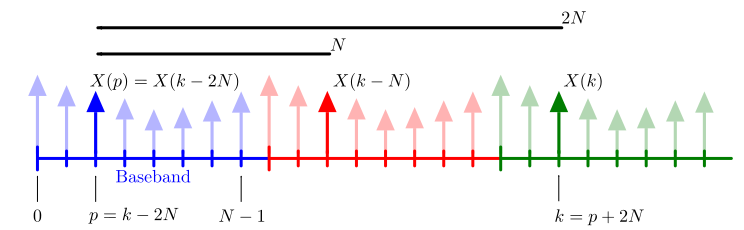
\includegraphics[width=\textwidth]{baseband.pdf}
\par\end{centering}
\caption{Illustration of the baseband and higher bands.}
\label{fig:baseband}
\end{figure*}


\subsubsection{DFT of a baseband complex exponential}

The DFT of an exponential is of fundamental importance.
Given a signal $x(n)=\exp(i2\pi nq/N)$ with $q$ in the baseband, the DFT value at a frequency $k$ in the baseband is
\begin{align}
X(k) =& \sum_{n=0}^{N-1} e^{i2\pi nq/N}e^{-i2\pi nk/N} \\
=& N \delta_{k, q} \, .
\end{align}
Of course, as already discussed, the DFT value for $k$'s outside the baseband are uniquely determined by those in the baseband.
In particular, in this case we have
\begin{equation}
X(k + mN) = N \delta_{k, q} \, .
\end{equation}
This is a series of delta peaks separated from each other by $N$ units in frequency space.
Note that this agrees with our previous discussion which said that all DFT coefficients separated by $N$ must be equal.
As previously explained, it makes sense to ignore the coefficients for $k$ outside the baseband, in which case the DFT of the exponential becomes
\begin{equation}
X(k) = \delta_{k,p} \label{eq:dftExponential}
\end{equation}
where $p$ is the \emph{unique} integer in the baseband which is related to $q$ by translation by an integer multiple of $N$, ie. $p=q-mN$.

\subsubsection{Aliasing}

What happens if we have an exponential signal $x(n)=e^{i2\pi nq/N}$ when $q$ is outside the baseband?
According to (\ref{eq:dftExponential}) we get a delta peak $\delta_{k,p}$ with $p$ in the baseband and $p = q-mN$ for some integer $m$.
The value of $m$ doesn't matter, the point is that an exponential at a frequency $q$ outside the baseband has the same DFT as an exponential with Fourier frequency $p$ inside the baseband.
A consequence is that if you measure a signal $A\exp\left[i2\pi nq/N\right]+B\exp\left[i2\pi n(q+mN)/N\right]$ the DFT will look exactly the same as if you had measured $(A+B)\exp\left[i2\pi nq/N\right]$.
The indistinguishability of these signals is called $\textbf{aliasing}$, because the actual signal at higher frequency $q+mN$ \emph{looks} like the lower frequency $q$ in frequency space.
What's going on here is that signals with Fourier frequency outside the baseband oscillate more than once per data point, but since we only sample once per data point these oscillations are hidden and the DFT sees the signal at a lower frequency.

In calculations it can be annoying to replace $q$ values outside the baseband by $p+mN$ explicitly.
Instead, you can just do the replacement once the computation is complete.
To get this right use the following \textbf{rules for computing DFTs}
\begin{equation}
\left[ \textrm{DFT}\left( e^{i2\pi nq/N} \right)\right](k) = \delta_{k,q} \, .
\end{equation}
Then, if $q$ is outside the baseband, at the end of the calculation find the corresponding $p$ inside the baseband and make the replacement
\begin{equation}
\delta_{k,q} \rightarrow \delta_{k,p} \quad q=p+mN \, . \label{eq:aliasReplacement}
\end{equation}


\section{Physical Frequencies}

Our mathematical time series was parametrized by only the number of points $N$. Physically, however, we have another parameter associated to the time series, the total time spanned by the experiment $T$, or equivalently either the time step between points $\Delta t$, or its inverse, the sampling rate $f_{\textrm{s}}$. These quantities are related by
\begin{displaymath}
T = N\Delta t = \frac{N}{f_{\textrm{s}}}
\end{displaymath}
So that only $N$ and one of the three equivalent time scales are independent.

A data point at time $t$ is given by $x(n=t/\Delta t)$. We use this formula to go between the purely mathematical formulas involving $N$ to those involving physical quantities. Using these relations we can re-express an exponential at Fourier frequency $k$ as
\begin{displaymath}
\exp \left(i2\pi\frac{nk}{N}\right) = \exp\left(i 2 \pi \frac{tk}{\Delta t N} \right) = \exp \left( i 2\pi t\frac{k}{T} \right)
\end{displaymath}
It is now clear that the physical Fourier frequencies are $k/T$, and since $k$ goes in integer steps the frequency resolution is $1/T$. This means that the frequency resolution of our transform is determined by the total measurement time. Longer measurement time gives better frequency resolution. This also means that the lowest frequency we can measure above DC is $1/T$.

To summarize, the physical frequencies that result in a DFT performed on a time series with $N$ points taken over a total time $T$ are
\begin{displaymath}
\frac{1}{T}\left[0,1,\ldots,N-1\right]\quad\textrm{or}\quad\frac{f_{s}}{N}\left[0,1,\ldots,N-1\right]
\end{displaymath}

\section{Example}

We now give an example to tie everything together. Consider a signal
\begin{displaymath}
s(t) = \exp (i 2\pi f t)
\end{displaymath}
for $f=120\textrm{Hz}$, and imagine we measure it for one second with one hundred sample points,
\begin{displaymath}
N=100 \qquad T=1\mathrm{s}
\end{displaymath}
The sampled function is
\begin{displaymath}
s(n) = \exp(i2\pi fnT/N) = \exp(i2\pi 120n/N)
\end{displaymath}
The DFT is simply $X(k)=\delta_{k,120}$, but since the baseband only runs from 0 to 99, the result is aliased and we pick up the signal at $k=20$, or in frequency units $f=20/T=20\mathrm{Hz}$. Note that if we somehow knew that the signal only had frequency components in the range say from 100Hz to 150Hz, then we would be able to interpret the DFT peak at 20Hz as the alias of the real signal at 120Hz. That's how aliasing works: if you have knowledge about where your signal might be, then you can figure out where the DFT weight is coming from, but otherwise you only know that there's signal at one of the equivalent frequencies from the various Brillouin zones. Signal analysis equipment generally deals with this problem by filtering the input so that it's guaranteed that the incoming signal resides only in the baseband. Of course, in real life you don't have complex signals (unless you're using an IQ mixer!) so the situation is a little different. This explained in the next section.

\section{The Nyquist frequency}

Next we consider the maximum measureable frequency. The maximum value of $k$ is $N-1\approx N$. This suggests that the maximum measured frequency in index units is
\begin{displaymath}
f_{max}=\frac{k_{max}}{N}=\frac{N}{N}=1
\end{displaymath}
ie, the maximum measured frequency corresponds to an exponential that goes through 1 cycle per index. In physical units this frequency is given by
\begin{displaymath}
f_{max}=\frac{\text{1 cycle}}{\text{index}}\rightarrow\frac{\text{1 cycle}}{\Delta t}=f_{s}
\end{displaymath}
which says that the maximum measured frequency is just the sampling frequency. This is wrong. There are several different ways of understanding why, but it is essentially due to the fact that all of the signals we measure in the lab are made up of real numbers. Real sines and cosines have $\emph{negative}$ frequency components which are outside the baseband, and this leads to aliasing.

It turns out that the maximum measurable frequency is actually $f_s/2$, or $N/2T$ in index units. This frequency, located halfway up the baseband, is called the \textbf{Nyquist frequency}. To understand this we compute the DFT of a cosine signal. Take $x(n)=A\cos (2\pi nq/N+\phi)$ with $q$ in the baseband and compute the DFT coefficients,
\begin{eqnarray*}
x(n) & = & A\cos\left(2\pi nq/N+\phi \right)\\
x(n) & = & \frac{A}{2}\left[e^{i\phi}e^{i2\pi nq/N}+e^{-i\phi}e^{-i2\pi nq/N}\right]\\
\text{so}\qquad X(k) & = & \frac{AN}{2}\left[e^{i\phi}\delta_{k,q}+e^{-i\phi}\delta_{k,-q}\right]\\
X(k) & = & \frac{AN}{2}\left[e^{i\phi}\delta_{k,q}+e^{-i\phi}\delta_{k,N-q}\right]\end{eqnarray*}
We have weight at $q$ and, because of the negative frequency, also at $N-q$. The negative frequency component of the sinusoid has been aliased! Now compare this to the DFT of a sinusoid at $N-q$, $y(n)=\cos(2\pi n[N-q]/N)$,
\begin{eqnarray*}
y(n) & = & A\cos\left(2\pi n[N-q]/N+\phi\right)\\
y(n) & = & \frac{A}{2}\left[e^{i\phi}e^{-i2\pi nq/N}+e^{-i\phi}e^{i2\pi nq/N}\right]\\
\text{so}\qquad Y(k) & = & \frac{AN}{2}\left[e^{i\phi}\delta_{k,q}+e^{-i\phi}\delta_{k,-q}\right]\\
Y(k) & = & \frac{AN}{2}\left[e^{i\phi}\delta_{k,q}+e^{-i\phi}\delta_{k,N-q}\right]
\end{eqnarray*}
Because of the aliased terms, $X(k)$ and $Y(k)$ are identical, even though they come from cosines at different frequencies which are \emph{both in the baseband}. Each cosine shows up at the ``correct'' frequency and also at an aliased frequency which is the reflection of $q$ about the Nyquist frequency. The upshot is that when you're dealing with real time signals, their complex form always has negative frequency components which are aliased by the DFT. Therefore, the lower and upper halves of the baseband are dependent on one another. The exact dependence is a complex conjugate symmetry. You can easily prove for any \textbf{real time series} $x(n)$,
\begin{equation}
X(k)^* = X(N-k) \label{eq:conjugateSymmetry}
\end{equation}
Therefore, only half of the baseband contains unique information, as manifest in our examples $x(n)$ and $y(n)$.

The situation is now that only the first half of the baseband is uniquely determined. Therefore, in order to ensure that a DFT is a faithful representation of the measured time series, one must be sure that the measured signal has frequency components no higher than the Nyquist frequency. If this condition is satisfied, then the DFT coefficients found in the lower half of the baseband exactly match those present in the original signal \footnote{Actually, in this case it's possible to reconstruct the \emph{continuous} time signal just from the DFT coefficients. This fact is sometimes referred to as the Shannon Sampling Theorem. A nice proof is given in the optics book by J. Goodman.}. Of course if you know that the signal's frequency components are contained entirely in just the upper half of the baseband, then the coefficients in the lower half are still a faithful representation if you take into account the reflection and complex conjugate symmetry.

In practice, signal processing equipment usually uses a lowpass filter on the input to kill off everything above the Nyquist frequency. This is called an \textbf{anti-aliasing filter}. In that case, the lower half of the baseband can be read off without worrying about aliasing.


\section{Power Spectrum}

We now finally come to the computation of physical power spectra. The question is, if we sample a real time signal and then compute the DFT, how do we turn this into a physical power spectrum? To find the answer we just compute the DFT of a real sinusoid and compare it to the known power of a sinusoid. Consider the signal $x(t) = A \cos (2 \pi f t)$ where $f$ is in the baseband and corresponds to the Fourier frequency $q$. Such a signal has total power $P=A^2/2$. If the signal has a finite linewidth $B$ then the power spectral density would be $S=A^2/2B$. This is the known reference against which we compare the result of the DFT. We already computed the DFT of a cosine with the result
\begin{displaymath}
X(k) = \frac{AN}{2} \left[ \delta_{k,q} + \delta_{k,N-q} \right]
\end{displaymath}
Since the power spectrum doesn't depend on phase, and should be proportional to $A^2$ it's clear that we should take the modulus square,
\begin{displaymath}
|X(k)|^2 = \frac{A^2N^2}{4} \left[ \delta_{k,q} + \delta_{k,N-q} \right]
\end{displaymath}
Throw out the aliased component since it doesn't have any extra information. Then, in order to get rid of the $N$ dependence and to get the correct numerical factor, multiply by $2/N^2$,
\begin{displaymath}
\frac{2}{N^2}|X(k)|^2 = \frac{A^2}{2} \delta_{k,q}
\end{displaymath}
A spectral density $S$ should have the property that $S$ multiplied by a span in frequency space gives the correct total power. The real frequency span between each point in DFT frequency space is $1/T$, so the total power ought to be $P=\frac{1}{T}\sum_k S(k)$. Applying this formula to our expression so far yields
\begin{displaymath}
\frac{1}{T}\frac{2}{N^2}\sum_k |X(k)|^2 = \frac{1}{T}\frac{A^2}{2}
\end{displaymath}
This differs from the correct power by a factor of $1/T$. Therefore, the correct power spectral density is
\begin{equation}
S(f) = \frac{2T}{N^2}|X(k=fT)|^2 \label{eq:powerSpectralDensity}
\end{equation}
Equation (\ref{eq:powerSpectralDensity}) is our most important result. It tells you how to convert from a DFT computed from a measured time series, to a physical power spectral density. Note that the units are exactly what they should be, $A^2/\textrm{Hz}$. This formula is only exactly correct if you can be sure that there is no aliasing contaminating the baseband. If this is not the case, then the spectral density you compute at a given frequency will be different from what was actually at that frequency. If the measured signals are coherent then the measured spectral density may be too low or too high. If the signal is noise, then the computed spectral density will always be greater than what actually existed in the measured signal.


\section{Noncommensurate Frequencies}


\subsection{Power in an exponential}

So far we've only talked about signals that are periodic in the time that we measure, ie. we've dealt with sinusoids of the form $\exp\left(2\pi nq/N\right)$. What happens if we have a sinusoid at an arbitrary frequency that is not one of the Fourier frequencies? To get an idea let's compute the Fourier series for a noncommensurate exponential, $\exp\left(i2\pi\xi x\right)$
\begin{align*}
f_{k} & = \int_{0}^{1}e^{-i2\pi kx}e^{i2\pi\xi x}\, dx\\
f_{k} & = \frac{\exp\left(i2\pi(\xi-k)\right)-1}{i2\pi(\xi-k)}\\
f_{k} & = \exp\left(i2\pi(\xi-k)/2\right)\frac{e^{i2\pi(\xi-k)/2}-e^{-i2\pi(\xi-k)/2}}{i2\pi(\xi-k)}\\
f_{k} & = \exp\left(i2\pi(\xi-k)/2\right)\textrm{sinc}\left(\xi-k\right)\\
|f_{k}|^{2} & = \textrm{sinc}^{2}\left(\xi-k\right)
\end{align*}
where $\textrm{sinc}(x)=\sin\left(\pi x\right)/\pi x$. To understand what this means, start by considering what happens if $\xi$ is an integer. If $\xi$ is an integer then $\exp\left(i2\pi\xi x\right)$ is commensurate on $[0,1]$ and the Fourier series has only one nonzero term, since the sinc function is zero for all integer arguments except 0. Therefore, in the case $f_{k}=\delta_{k,\xi}$. However, if $\xi$ is not an integer then the Fourier series is nonzero for all $k$.

The case of a DFT essentially the same thing happens. Let's see this explicitly by computing the DFT, \footnote{To compute the finite sum we use the formula $1+x+x^{2}+\cdots+x^{N-1}=(x^{N}-1)/(x-1)$.}
\begin{align*}
X(k) & = \sum_{n=0}^{N-1}e^{-i2\pi nk/N}e^{i2\pi n\xi/N}\quad\xi\textrm{ not an integer}\\
X(k) & = \sum_{n=0}^{N-1}\left[e^{i2\pi(\xi-k)/N}\right]^{n}\\
X(k) & = \frac{\exp\left[i2\pi\left(\xi-k\right)\right]-1}{\exp\left[i2\pi\left(\xi-k\right)/N\right]-1}\\
X(k) & = e^{i\pi(\xi-k)(N-1)/N}\frac{\sin\left(\pi\left(\xi-k\right)\right)}{\sin\left(\pi\left(\xi-k\right)/N\right)}\\
|X(k)|^{2} & = \left(\frac{\sin\left[\pi\left(\xi-k\right)\right]}{\sin\left[\pi\left(\xi-k\right)/N\right]}\right)^{2}
\end{align*}
This says that the power is spread out over several values of $k$ just like in the Fourier series case. In Figure 1 we show the numerically computed $|\textrm{DFT}|^2$ of a noncommensurate exponential along with the expected curve.


\quickfig{\columnwidth}{leakage.pdf}
{Numerically computed DFT (power) of a noncommensurate exponential
with theory curve. The signal is $\exp\left[i2\pi n\xi/N\right]$
with $N=20$ and $\xi=12.2$. The mod square of the DFT is shown in
blue and the theory curve is in red.}
{Flo:leakage}


\subsection{Power in sinusoids}

\subsubsection{Fourier Series}

Consider a signal over a finite interval given by $s(x)=\cos(2\pi\xi x)$
where $x\in[0,1]$. Note that $\nu$ is the number of oscillations
of the signal over the sampled interval. The power in this signal
is \begin{eqnarray*}
P & = & \int_{0}^{1}s(t)^{2}dx\\
P & = & \int_{0}^{1}\cos(2\pi\xi x)^{2}dx\\
P & = & \frac{1}{2}\left[1+\textrm{sinc}\left(4\xi\right)\right]\end{eqnarray*}
This curve is plotted in Figure \ref{Flo:PowerFromNoncommensurateSinusoid}.

%
\begin{figure}
\begin{centering}
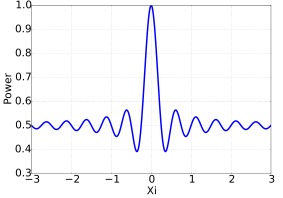
\includegraphics[width=8cm]{power.pdf}
\par\end{centering}

\caption{Measured power in a sinusoid with $\xi$ cycles over the measurement
time. Note that away from DC the power is nearly $1/2$ as appropriate
for an infinitely long sinusoid. Note also that commensurate sinewaves
give exactly $1/2$.}


\label{Flo:PowerFromNoncommensurateSinusoid}
\end{figure}


It would be nice to see explicitly that this strange power curve is
reproduced in frequency space. To do this, we will compute the Fourier
Series for the signal, and then sum the squares of the Fourier coefficients
to see if we get this same total power. The Fourier coefficients for
the sinusoid are computed easily because we already worked them out
for exponentials,\begin{align*}
s(t) & = \cos(2\pi\xi x)\\
s(t) & = \frac{1}{2}\left[e^{i2\pi\xi x}+e^{-i2\pi\xi x}\right]\\
s_{k} & = \frac{1}{2}\left[e^{i\pi(\xi-k)}\textrm{sinc}\left(\xi-k\right)+e^{-i\pi(\xi+k)}\textrm{sinc}\left(\xi+k\right)\right]\\
|s_{k}|^{2} & = \frac{1}{4}\left[\textrm{sinc}\left(\xi-k\right)^{2}+\textrm{sinc}\left(\xi+k\right)^{2}+\right.\\
 & + \left.2\cos\left(2\pi\xi\right)\textrm{sinc}\left(\xi-k\right)\textrm{sinc}\left(\xi+k\right)\right]
\end{align*}
The total power should be $\sum_{k=-\infty}^{\infty}|s_{k}|^{2}$,
so to check for consistency we need to do the sum over $k$. The necessary
sums are done explicitly in appendix ??, and the result is that\[
\sum_{k=-\infty}^{\infty}|s_{k}|^{2}=\frac{1}{2}\left[1+\textrm{sinc}\left(4\xi\right)\right]\]
in agreement with the time domain integral. This is an important result.
It means that 


\subsubsection{DFT}

Frequently one wants to determine the amount of power at each frequency
in an experimentally obtained time series. To find out how to get
this, let's consider a cosine wave\[
s(t)=A\cos\left(2\pi ft\right)\]
 The power in this signal is $A^{2}/2$. What happens when we sample
the signal and compute the DFT? The sampled signal can be written
as\begin{eqnarray*}
s(n) & = & A\cos\left(2\pi fn\cdot\delta t\right)\\
s(n) & = & \frac{A}{2}\left[\exp\left(i2\pi fn\cdot\delta t\right)+\exp\left(-i2\pi fn\cdot\delta t\right)\right]\end{eqnarray*}
 where $\delta t$ is the sampling interval. Noting that $f\cdot\delta t=\xi/N$
we can take the DFT\begin{align*}
s_{k} & = \frac{A}{2}e^{-i\pi k(N-1)/N}\left[e^{i\pi\xi(N-1)/N}\frac{\sin\left[\pi\left(\xi-k\right)\right]}{\sin\left[\pi\left(\xi-k\right)/N\right]}+\right.\\
 & + \left.e^{-i\pi\xi(N-1)/N}\frac{\sin\left[\pi\left(\xi+k\right)\right]}{\sin\left[\pi\left(\xi+k\right)/N\right]}\right]\\
s_{k} & = \left(\frac{A}{2}\right)^{2}\left[\left(\frac{\sin\left[\pi\left(\xi-k\right)\right]}{\sin\left[\pi\left(\xi-k\right)/N\right]}\right)^{2}+\right.\\
 & + \left.\left(\frac{\sin\left[\pi\left(-\xi-k\right)\right]}{\sin\left[\pi\left(-\xi-k\right)/N\right]}\right)^{2}+\right]\\
|s_{k}|^{2} & = \frac{A^{2}}{4}\left[\frac{\sin\left[\pi\left(\xi-k\right)\right]}{\sin\left[\pi\left(\xi-k\right)/N\right]}+\frac{\sin\left[\pi\left(-\xi-k\right)\right]}{\sin\left[\pi\left(-\xi-k\right)/N\right]}\right]^{2}
\end{align*}



\section{Appendix - Sums for Fourier Series power analysis}

The sum we want to compute is\begin{eqnarray*}
S & = & \frac{1}{4}\sum_{k}\left[\textrm{sinc}(\xi-k)+\textrm{sinc}(\xi+k)\right.\\
 & + & \left.2\cos(2\pi\xi)\textrm{sinc}(\xi-k)\textrm{sinc}(\xi+k)\right]\end{eqnarray*}
We write this as\[
S=\frac{1}{4}\left[S_{1}+S_{1}+2\cos(2\pi\xi)S_{2}\right]\]
The first sum we need to do is\[
S_{1}=\sum_{k=-\infty}^{\infty}\textrm{sinc}(\xi-k)^{2}\]
This is easy if we use the Poisson summation formula which states
that\[
\sum_{n}f(n-\xi)=\sum_{m}\tilde{f}(m)e^{-i2\pi\xi m}\]
Using this formula we get\begin{eqnarray*}
S_{1} & = & \sum_{m}\widetilde{\textrm{sinc}^{2}\left(m\right)}e^{-i2\pi\xi m}\\
S_{1} & = & \sum_{m}\textrm{tri}(m)e^{-i2\pi\xi m}\end{eqnarray*}
where $\textrm{tri}(x)$ is a triangle function; ie, $\textrm{tri}(x)=x+1$
for $-1<x<0$ and $\textrm{tri}(x)=-x+1$ for $0<x<1$, and $\textrm{tri}(x)=0$
elsewhere. Since $\textrm{tri}(m)$ is only nonzero for $m=0$ the
sum is simply\[
S_{1}=1\]
The second sum we need to do is\[
S_{2}=\sum_{k=-\infty}^{\infty}\textrm{sinc}(\xi-k)\textrm{sinc}(\xi+k)\]
For now we just write $f$ instead of $\textrm{sinc}$ to tidy up
notation. Since $\textrm{sinc}$ is an even function we can stick
a minus sign in the first function like so,\[
S_{2}=\sum_{k}f(k-\xi)f(k+\xi)\]
From here we just crank,\begin{eqnarray*}
S_{2} & = & \sum_{k}\int_{q}\int_{q'}\tilde{f}(q)e^{i2\pi q(k-\xi)}\tilde{f}(q')e^{i2\pi q'(k+\xi)}\\
S_{2} & = & \int_{q}\int_{q'}\tilde{f}(q)\tilde{f}(q')e^{-i2\pi\xi(q-q')}\sum_{k}e^{i2\pi k(q+q')}\\
S_{2} & = & \int_{q}\int_{q'}\tilde{f}(q)\tilde{f}(q')e^{-i2\pi\xi(q-q')}\sum_{n}\delta(n-q-q')\\
S_{2} & = & \sum_{n}\int_{q}\tilde{f}(q)\tilde{f}(n-q)e^{-i2\pi\xi(2q-n)}\\
S_{2} & = & \sum_{n}e^{i2\pi\xi n}\int_{q}\tilde{f}(q)\tilde{f}(n-q)e^{i2\pi q(-2\xi)}\end{eqnarray*}
Now we have to pay attention to what $\tilde{f}$ actually is. It
turns out that the Fourier transform of the sinc function is simply
a constant function from -1/2 to +1/2 with unit amplitude. This means
that $\tilde{f}(q)\tilde{f}(n-q)$ is only nonzero for $n=0$, in
which case it is equal to $\tilde{f}(q)$. Therefore we get\begin{eqnarray*}
S_{2} & = & \int_{q}\tilde{f}(q)e^{i2\pi q(-2\xi)}\\
S_{2} & = & f(-2\xi)\\
S_{2} & = & \textrm{sinc}(-2\xi)\\
S_{2} & = & \textrm{sinc}(2\xi)\end{eqnarray*}
Plugging into the original expression gives\begin{eqnarray*}
S & = & \frac{1}{4}\left[1+1+2\cos(2\pi\xi)\textrm{sinc}(2\xi)\right]\\
S & = & \frac{1}{2}\left[1+\cos(2\pi\xi)\textrm{sinc}(2\xi)\right]\\
S & = & \frac{1}{2}\left[1+\textrm{sinc}(4\xi)\right]\end{eqnarray*}
as stated in the main text.
\end{document}
